%%%%%%%%%%%%%%%%%%%%%%%%%%%%%%%%%%%%%%%%%%%%%%%%%%%%%%%%%%%%%%%%%%%%%%%%%%%%%%%%%%%%%%%%%%%%%%%%%%%%%%
%
%   Filename    : chapter_1.tex 
%
%   Description : This file will contain your Research Description.
%                 
%%%%%%%%%%%%%%%%%%%%%%%%%%%%%%%%%%%%%%%%%%%%%%%%%%%%%%%%%%%%%%%%%%%%%%%%%%%%%%%%%%%%%%%%%%%%%%%%%%%%%%

\chapter{Introduction}
\label{sec:intro}    %--note: labels help you with hyperlink editing (using your IDE)

This chapter gives an overview of the purpose of our study and the motivations for pursuing it. We outline our goals, limitations, and the methods that we intend to use in our research.

%%This chapter builds the motivation for the conduct of the research through a description of the background of the study or the current state of technology. This is followed by the research objectives, the scope and limitations, and significance of the research. The chapter ends with the research methodology describing the different activities to be conducted to achieve the goals of this research.%%


%%
%% --- 1.1 Background of the Study --- %%
%%

\section{Background of the Study}
\label{sec:overview}

%
%   NOTE: You have to delete/replace the unnecessary paragraphs with your own text.
%


%%This section gives the reader an overview of the specific technology or field in the international or local setting. The information regarding the technology or field should be contemporary and not
%%based on outdated sources. Discussion must not be too technical or too detailed.

%%Follow the inverted pyramid to describe each of the following. Allocate one (1) paragraph per level in the pyramid. 

% Describe the research area
%Research area ...
%This study's main research area is on personality computing. Personality computing is related to artificial intelligence and personality psychology by studying one's personality through a variety of computational techniques from different sources (usually text, multimedia, and social networks). Among the three main problems personality computing addresses; automatic personality recognition, perception, and synthesis \citep[p.~280]{Vinciarelli2014}; this study focuses on automatic personality recognition.

% Describe the domain (where will you apply the topic)

Personality is defined as “patterns of thought, emotion, and behavior” \citep{Vinciarelli2014}. For purposes of personality computing, personality is broken down into various characteristics that can be measured quantitatively \citep{Vinciarelli2014}. The most widely used model in this field is the Big Five Personality Model, which comprises the traits of extraversion, agreeableness, conscientiousness, neuroticism, and openness. Other well-known models include the Myers–Briggs Type Indicator (MBTI) and the Cattell Sixteen Personality Factor (16PF). Using these models, the traditional method of measuring personality is by using a multiple-choice questionnaire \citep{farnadi2018}, wherein each choice corresponds to a value for each personality characteristic. These values are then aggregated to obtain the final results, which may take the form of numerical scores for each trait or categorical classifications. Understanding personality plays a significant role in fields such as psychology, as this information can be used in studies of mental health and human behavior. It has also garnered increasing interest in the fields of social science, business, education, and healthcare \citep{Miller2014} as it offers valuable insights into individual differences and supports more personalized approaches in these domains.

However, these traditional methods of identifying personality are time-consuming and may be inconvenient for participants \citep{chen2016}, prompting the need for alternative methods to obtain these results. This leads us to the field of Automatic Personality Recognition (APR). APR aims to infer an individual’s personality based on their digital footprint. APR has been traced back to the work of \citet{Pennebaker1999} wherein they asked the question of \textit{can language use reflect personality style?} APR studies typically use inputs such as text, audio, or visual data, along with an individual’s personality trait scores, to train machine learning models. These models aim to analyze patterns and identify correlations in order to form accurate personality predictions, which may be either categorical or continuous (regression-based) in nature.

% Give a synthesis of previous work

% Synthesis of previous studies...
%\citet{Pennebaker1999} and \citet{Mairesse2007} had demonstrated the different ways of detecting personalities and emotions by analyzing the text with various language models. Due to that, social media had became a common place for the research of personality detection. The PagkataoKo dataset has been made with social media activity on Instagram and X (formerly known as Twitter). There were more studies using X's data than Instagram due to X being a more prominent platform with its text-based posts. However, \citet{ferwerda2016}, \cite{Reece2017-qw} and \cite{Harris2019-gq} made studies that showed analyzing photos was possible. Thus, researching on Instagram became more meaningful in this manner.

Early studies in APR predominantly focused on text-based features, and more recent work has expanded to include multimodal data, such as images and videos \citep{Mehta2020}, reflecting the evolving nature of online content. The standard approach involves feature extraction, followed by machine learning techniques to associate extracted features with personality traits. Support vector machines (SVMs) are commonly used in APR studies. However, many have also found success with deep learning approaches \citep{Zhao2022} such as deep neural networks (DNNs), convolutional neural networks (CNNs), and recurrent neural networks (RNNs).

With the widespread adoption of social networking sites (SNS), personal content such as images, captions, and interactions has become publicly available on a large scale, providing accessible behavioral data for personality analysis and greater opportunity for research. Prior research suggests that user-generated content on these platforms often reflects personal expression in spontaneous and unintended ways \citep{Vinciarelli2014}, making them valuable for computational personality inference. Thus, many studies have taken to conducting personality analysis using data from personal social media profiles. Text was a common modality in their research, though a smaller number of papers have also explored image-based analysis. 

Most existing APR studies have predominantly focused on Western populations, but progress in APR studies of non-Western languages is slowly being made, including Filipino. Filipino APR is a growing subfield that has started to gain increasing interest. This area presents unique challenges, such as frequent code-switching and the presence of diverse regional languages \citep{tighe_acorda_2022}. However, existing studies in this field have primarily focused on either the activity and usage of social media itself or on a text-based linguistic analysis of social media posts made by Filipinos in order to predict personality. There is a heavier focus on textual data as a modality, particularly X (formerly Twitter) data, while image-based and multimodal approaches remain largely underexplored. Platforms like Instagram offer a rich source of multimodal data, specifically images and text, that could notably improve personality analysis \citep{Skowron2016}. Furthermore, numerous studies show improved performance when multiple modalities are analyzed over just a single modality \citep{batrinca_multimodal_2016, lima_sequential_2022}. This presents the opportunity to explore a multimodal approach to Filipino APR using Instagram image data in addition to text data, which has the potential to improve upon existing models and yield more accurate results.

% State the problem and the research question

% Paragraph containing the Problem Statement or the Research Question.

This study seeks to explore multimodal APR methods tailored for Filipino users by leveraging Instagram data, integrating psychological analysis and computational techniques. The study aims to address the question: \textit{How effective is multimodal Instagram data as a source for recognizing manifestations of Filipino personality traits?}

% This section ends with a discussion on the problem/s faced by or that still exist in the specific technology or field (e.g., limitations of existing software or algorithms). It should not contain your research objectives or goal; instead, the problem statement would lead to the research objectives to be stated in 1.2.

% \subsection{Figures}

% Often times, a graph, illustration, screenshot, or any image can help a reader better understand what we say in text. In academic writing, we call them \textbf{figures}. Please add as many figures as necessary to help build your narrative, but do not go overboard. 

% You can add figures in JPG or PNG format as shown in Figure \ref{fig:disneystock}. All figures should also have a descriptive caption. As a general principle, your caption should adequately describe what is shown in the figure, and not just short texts. If we remove all the surrounding text, the reader should still understand what your figure is. 

% All figures should be referred to at least once in the surrounding paragraphs. Make sure that you explain what the figure is all about, and that you refer to your figure. You can also use the surround paragraphs to highlight key insights or parts of your figure. For example, \figref{fig:disneystock} shows a graph of the performance of Disney stock from the 1980s to 2012.

% %--- the following example shows how to include a figure in PNG format
% \begin{figure}[t]                %-- use [t] to place figure at top, [b] to place at the bottom, [h] for here
%    \centering                    %-- use this to center the figure
%    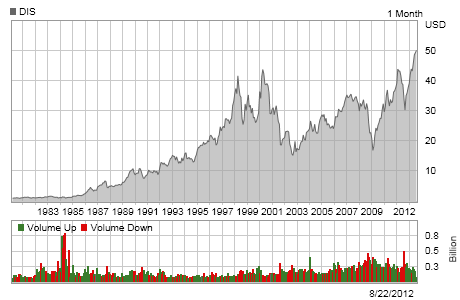
\includegraphics{DisneyChart.png}      %-- include image file named as "disneychart.png" 
%    \caption{Disney's stock price chart from the 1980s up to 2012. The top chart shows the stock price in each month. The bottom chart shows the change in volume of transactions. The bars are colored based on the type of movement that happened in a month.}
%     \label{fig:disneystock}
% \end{figure}

% \subsection{References}

% Some notes on citing references. When using APA format, the author-date method of citation is followed. This means that the author's last name and the year of publication for the source should appear in the text, and a complete reference should appear in the reference list.

% %
% % Examples:
% %     	Smith (1970) compared reaction times . . .
% %     	In a recent study of reaction times (Smith, 1970), . . .   
% %     	In 1970, Smith compared reaction times . . .
% %	Smith, et al., (1970) compared reaction times . . .
% %     	In a recent study of reaction times (Smith, et al., 1970), . . .  
% %     	In 1970, Smith, et al., compared reaction times . . .
% %

% Here are some examples on how to do the referencing (note author's name and years are different from commented examples). For APA citation details, refer
% to \url{http://www.ctan.org/tex-archive/biblio/bibtex/contrib/apacite/}. 

% \begin{itemize}
%  \item \citeA{kartch:2000:ERA} compared reaction times...
%  \item In a recent study of reaction times \cite{kartch:2000:ERA}...
%  \item In \citeyearNP{kartch:2000:ERA}, \citeauthor{kartch:2000:ERA} compared reaction times...
%  \item \shortciteA{fedkiw:2001:VSO} compared reaction times... 
%  \item In a recent study of reaction times \cite{fedkiw:2001:VSO}...
%  \item In \citeyearNP{fedkiw:2001:VSO}, \shortciteauthor{fedkiw:2001:VSO}, compared reaction times...
% \end{itemize}

% The following are references from journal articles \cite{Park:2006:DSI, Pellacini:2005:LAH, sako:2001:SSB}.  Here's an MS thesis document \cite{yee:2000:SSA}, and this is from a PhD dissertation \cite{kartch:2000:ERA}. For a book, reference is given as \cite{parke:1996:CFA}.  Proceedings from a conference samples are \cite{Jobs95, fedkiw:2001:VSO,levoy:2000:TDM}.  

% The sample bibliography file named \textbf{myreferences.bib} is from the
% SIGGRAPH \LaTeX template.  You can use a text editor to view the contents of the bib file. It is your task to create your own bibliography file.  For those who downloaded papers from ACM or IEEE sites, there is a BibTeX link that you can click; thereafter, you just simply need to copy and paste the BibTeX entry into your own bibliography file.

% \subsection{Code snippet}

% The following shows how to include a program source code (or algorithm). The verbatim environment, as the name suggests, outputs text (including white spaces) as is...

% \begin{verbatim}
%                #include <stdio.h>
%                main()
%                {
%                     printf("Hello world!\n");
%                }
% \end{verbatim}


%%
%% --- 1.2 Research Objectives --- %%
%%

\section{Research Objectives}
\label{sec: objectives}
This study aims to explore the effectivity of a multimodal approach using Instagram data in the study of Filipino Automatic Personality Recognition. To achieve this, the study will pursue the following specific objectives:

\begin{enumerate}
	\item To determine and finalize the subset of data points to be used from the Instagram portion of PagkataoKo dataset.
 
	\item To identify data characteristics of the Instagram subset of the PagkataoKo dataset that are relevant to APR.

	\item To perform image and text feature extraction on the dataset based on previously identified characteristics.

	\item To build personality prediction models using different feature sets and machine learning algorithms.

 	\item To identify which visual or textual features are most indicative of certain personality traits.

	\item To evaluate the performance of the models using various metrics and compare the results to existing unimodal approaches.
\end{enumerate}

% This subsection states the over--all goal that must be achieved to answer the problem. Address the following: Given your research challenge or opportunity, how do you intend to solve it? What is the main outcome of your research? What kind of contribution do you want to achieve?

% The \textbf{general objective} is broken down into three or more specific objectives. The \textbf{specific objectives} are relatively smaller objectives that help you attain your general objective. You can formulate your specific objectives based on your running questions about the project. For example, the group does not have a good picture yet of the different conversation patterns between humans that can be mimicked by conversational agents. A specific objective can be "to identify different human-human conversation patterns." These objectives must be specific, measurable, attainable, realistic, and time-bounded.

% Reviewing related literature, studying a particular programming language or development tool (e.g., to study Windows/Object-Oriented/Graphics/C++ programming), and documentation to accomplish the general objective is inherent in all thesis projects and, therefore, must not be included here.


\begin{comment}
%
% IPR acknowledgement: the following sentences and examples are from Ethel Ong's slides 
%     on Research Objectives
%

How to formulate your research objectives:
1. Identify what research steps do you need to perform to achieve your general objective.
2. Identify the questions that must be answered for you to achieve your general objective.
    Thereafter, convert these questions into action statements


Example #1:

Question:
    What strategies do human educators employ in collaborative storytelling with children?

Specific Objective:
   To review existing strategies employed by language educators when sharing storytelling with children


Example #2:

Question:
   How will you represent commonsense knowledge for use by computer systems?

Specific Objective:
   To identify knowledge representation approaches used by existing story generation systems

Example #3:
Question:
   What types of storytelling knowledge are needed to generate stories?

Objective:
    To identify the different types of storytelling knowledge used in generating stories

Example #4:
Question:
    What machine learning approaches will you utilize?

Specific Objective:
    To determine existing machine learning algorithms [that can be used in training the computer system to detect cyberbullying cases] 

Example #5: 
Question:
    How will your research output be evaluated?

Specific Objective:
    To define evaluation metrics for validating the accuracy of the translation
\end{comment}


%
%  The following is the format for presenting your specific objectives; replace them with your own 
%

% The specific objectives of this research are as follows:
% \begin{enumerate}
%    \item To identify knowledge representation approaches used by existing story generation systems;
%    \item To identify the different types of storytelling knowledge used in generating stories;
%    \item To build a neural-based model for generating events comprising a story; and
%    \item To define evaluation metrics for evaluating the performance of the event generation model.
% \end{enumerate}


%%
%% --- 1.3 Scope and Limitations --- %%
%%

\section{Scope and Limitations of the Research}
\label{sec:scopelimitations}


	This study aims to develop a multimodal personality recognition framework that predicts Filipino Instagram users’ Big Five personality traits using both image and text data. The following outlines the scope, limitations, and rationale for each research objective.
	\subsection{Perform exploratory data analysis (EDA) on the dataset}
	
	EDA is essential to understand the dataset’s structure, distribution, and quality. It helps uncover patterns, inconsistencies, and potential biases within Instagram images and captions, informing subsequent feature extraction and modeling processes.
	
	The study focuses exclusively on Instagram posts that contain both images and captions to ensure suitability for multimodal analysis. Posts lacking either modality are excluded. Social interaction metrics such as likes, comments, and follower counts are beyond the scope, as the study emphasizes content based personality signals, not engagement behaviors.
	
	\subsection{Structure and extract features from the image and text data}
	
	Social media data is inherently unstructured and cannot be directly used for personality trait prediction. Preprocessing and feature extraction are required to convert images and captions into structured, machine readable formats that capture relevant personality related cues.
	
	The study will process captions in any language, including English, Filipino, regional dialects, or other languages that may be present in the dataset. The presence of multiple languages is acknowledged as a natural characteristic of Filipino Instagram use, particularly given code switching tendencies and the multicultural linguistic environment. However, the primary analytical focus remains on English and Filipino captions, as these are the most prevalent based on prior research and the PagkataoKo dataset. Emojis, hashtags, and links will be minimally cleaned but retained as meaningful tokens (e.g., links will be tokenized as “[LINK]”), recognizing their relevance in expressing personality and emotion.
	
	The study recognizes that Instagram is a highly visual platform, and the images shared by users offer rich, often spontaneous cues that can be indicative of personality traits. To effectively extract relevant information, this research employs a two pronged image processing approach.
	
	For Photo Characteristics Analysis, this aspect focuses on the low level visual properties of the images, which previous studies have shown to correlate with personality traits. Specifically, dominant colors will be identified using color space transformations such as HSV color space and clustering techniques like k-means clustering. Prior research has found associations between image color and Big Five traits. For example, \cite{Branz2020} observed that warmer hues such as red and orange were more common in images posted by individuals high in Openness, while cooler hues like blue were linked to higher levels of Conscientiousness. This color-personality association aligns with findings by \cite{jue2022}, who reported a significant preference for green and blue tones among participants scoring high in Openness and Conscientiousness, respectively, although effect sizes were modest. These findings support the inclusion of color features (e.g., hue, brightness) as relevant indicators in image-based personality recognition. In addition, global image brightness and saturation levels will be computed, as these have been linked to traits such as Extraversion, which is associated with brighter, more saturated images, and Neuroticism, which is often reflected in darker, muted images. Image dimensions and resolution will also be recorded to account for possible differences in image quality or user posting behavior that may relate to personality traits.
	
	For Image Content Analysis, the semantic content of images provides higher level cues relevant to personality. Pretrained deep learning models, such as the Google Vision API or similar object recognition frameworks, will be used to identify objects, people, and common scenes present in the images. For example, frequent posting of selfies or group photos may indicate higher levels of Extraversion, while nature scenes or artistic compositions may signal Openness. Using algorithms such as OpenCV’s Haar cascades, the presence and quantity of faces in an image will also be detected. This serves as a proxy for social engagement tendencies, as prior research has linked higher face presence with Extraversion. Where possible, image metadata or contextual tags—such as inferred locations like beaches, cafes, or landmarks—will be utilized to enrich content understanding.
	
	All image features, both low level and high level, will be converted into structured, machine readable formats to be integrated with textual features in the multimodal personality recognition framework.
	
	\subsection{Train Machine Learning Models for Personality Trait Prediction
	}
	
	Model training operationalizes the proposed multimodal framework and enables empirical evaluation of its ability to predict personality traits based on extracted features.

	The models are limited to classification-based approaches to assign users to discrete personality categories. While previous studies in Filipino APR utilized regression models, their accuracy was low. Several studies identified by the researchers as relevant use classification models, which is an approach underrepresented in the Filipino context. Additionally, when it comes to real-world applications, service or product providers only care about whether scores are high or low, with the specifics not being important \citep{wei2017beyond}. Therefore, we chose to simplify the task by approaching it with a classification methodology since the nuance is not necessary.

	Support Vector Machines (SVM) and XGBoost will be utilized due to their strong performance and suitability for medium-scale datasets. A logistic regression (LR) model will be trained as a strong and interpretable baseline, which will provide a benchmark to compare against the more complex models. Deep learning models, though powerful, are excluded to ensure interpretability and mitigate overfitting risks, considering the dataset size.
	
	\subsection{Evaluate the predictive performance of the proposed multimodal framework}
	
	Evaluation determines whether integrating image and text data improves personality prediction compared to unimodal models.
	
	Evaluation is confined to within dataset testing using metrics such as Macro-F1 score and AUC-ROC. The study specifically targets Filipino Instagram users, limiting the generalizability of results to other populations, cultures, or platforms.
	

% This section discusses the boundaries, with respect to the objectives, of the research and the constraints within which the research will be developed. Describe what is and is not included in the scope of your research, supported by your main research question and findings of previous studies. Do not use weak excuses such as the lack of time and/or knowledge to perform the research.

% A good rule of thumb is to allocate one paragraph for each of your specific objectives that (1) contains a brief overview of the concept/theory and the purpose of doing the associated objective; and (2) includes a description of the scope/limitation of your study, and followed by brief purpose, rationale and/or justification for your decisions.

% The following should also be indicated in your Scope and Limitations (in the appropriate paragraphs matching the objectives, or as a stand-alone paragraph):
% \begin{itemize}
%    \item The profile and demographics of your target participants
%    \item Your data sources (i.e., new data, data from previous studies, data to be provided by some experts, data to be retrieved from social networks)
%    \item The specific technology platform to be utilized
%    \item The methods for collecting the data
%    \item The coverage areas or locations
%    \item The duration or time period (e.g., news articles for the year 2016-2017)
% \end{itemize}


%%
%% --- 1.4 Significance of the Research --- %%
%%

\section{Significance of the Study}
\label{sec: Significance}

The field of Filipino Automatic Personality Recognition (APR) is still emerging, presenting unique challenges due to the country’s linguistic diversity and rich cultural context. While progress has been made, existing research remains largely limited to unimodal approaches, particularly focusing on text based analysis. Most studies in the Filipino context, such as those utilizing the PagkataoKo dataset, rely heavily on linguistic features from Twitter or Instagram captions to infer personality traits. Although these studies have demonstrated some success, their predictive performance remains modest, and they often struggle to generalize across traits, especially for personality dimensions such as \textit{Openness} and \textit{Extraversion} that are more visually encoded.

Unimodal text based models have inherent limitations when applied to Filipino APR. The complex linguistic landscape, marked by code switching between English, Filipino, and regional dialects, alongside the informal and abbreviated nature of social media language, poses significant challenges to purely text based models. Moreover, platforms like Instagram emphasize visual expression, meaning that a large portion of users' self presentation and personality cues may not be adequately captured through text alone. Existing image only studies in broader APR research have shown that visual features, such as color schemes, image content, and aesthetics, carry significant personality signals, yet these have been largely underutilized in the Filipino context.

Given these limitations, this study seeks to advance Filipino APR by adopting a \textbf{multimodal approach}, integrating both image and text features from Instagram. Global research has consistently demonstrated that combining multiple modalities such as text, images, and metadata improves the robustness and accuracy of personality prediction models. However, this potential remains underexplored in Filipino APR, where studies have yet to systematically fuse visual and linguistic information for personality assessment.

In line with this, the study offers the following contributions:

\begin{itemize}
	\item It explores the use of multimodal data (image and text) for Filipino APR, addressing the current research gap and assessing whether this approach can meaningfully improve personality prediction.
	
	\item It acknowledges and addresses the complexities of Filipino linguistic expression, including:
	\begin{itemize}
		\item Code switching between English, Filipino, and regional dialects;
		\item The frequent use of emojis, hashtags, and links;
		\item Multimodal communication patterns prevalent on Instagram.
	\end{itemize}
	
	\item It conducts exploratory data analysis (EDA) on Filipino Instagram data to establish an empirical foundation for understanding content patterns relevant to personality traits.
	
	\item The research demonstrates practical methods for multimodal feature extraction and fusion, tailored to the Philippine social media landscape. This ensures that the methodologies account for both cultural and technological realities of how Filipinos express themselves online.
\end{itemize}

Beyond academic contributions, this study informs the development of culturally sensitive personality computing systems. By highlighting the importance of multimodal, localized approaches, it lays the groundwork for future research and applications that better reflect the linguistic, cultural, and behavioral patterns of Filipino social media users.

%%This section explains why research must be done in this area.  It rationalizes the objective of the research with that of the stated problem. Avoid including sentences such as ``This research will be beneficial to the proponent/department/college'' as this is already an inherent requirement of all BS and MS thesis projects.  Focus on the research's contribution to the Computer Science field.

%%The following are guide questions that may help your formulate the significance of your research. 


%
% IPR acknowledgement: the following list of items are from Ethel Ong's slides on Significance of the Research
%
%%\begin{itemize}
%%\item  What is the relevance and contribution of your work to the computer science community? 

\section{Ethical Considerations}
\label{sec:Ethics}

The methods involved in the creation of the PagkataoKo dataset were reviewed and approved by the Research Ethics Office of De La Salle University \citep{tighe_acorda_2022}. This approval ensures that the study adheres to established ethical standards for research involving human participants, particularly in the collection and handling of social media data.

\begin{itemize}
	\item \textbf{Data Compliance:}
	\begin{itemize}
		\item All volunteers provided informed electronic consent before their data was included in the dataset. This consent process outlined the scope, purpose, and limitations of the research.
		\item Data collection complied with the official developer policies and terms of service of both Twitter and Instagram, ensuring responsible and lawful data access through their respective APIs.
	\end{itemize}
	
	\item \textbf{Privacy Protection:}
	\begin{itemize}
		\item Personally identifiable information (PII), including \texttt{UserID} and account metadata, was fully anonymized to prevent the tracing of data back to individuals.
		\item All raw data, such as original posts and media files, were stored in encrypted form and restricted to authorized personnel only. This minimizes the risk of data breaches or unauthorized access.
	\end{itemize}
	
	\item \textbf{Data Restrictions:}
	\begin{itemize}
		\item The dataset is used strictly for academic research purposes and is not intended for any commercial exploitation.
		\item Reidentification of users is explicitly prohibited, and no attempts were made to reconstruct individual profiles or trace behavior back to specific persons.
	\end{itemize}
\end{itemize}

%%\begin{itemize} 
%%\item How does your technical contributions or empirical findings advance the field or grow our body of knowledge? 
%%\item If you built a prototype of an interaction technique, interface, library, tool, or system, what is value does it add compared to existing solutions? 
%%\end{itemize}

%%\item What will be your contributions to society in general? 
%%    \begin{itemize}
%%      \item How will your main stakeholders benefit from your technical contributions or empirical findings? 
%%      \item What are the positive social or economic impacts? 
%%%%   \end{itemize}
%%\end{itemize}

\begin{comment}
If applicable, describe possible commercialization and/or innovation in your research.
\end{comment}
